\documentclass[11pt, compress]{beamer}
\usepackage{amsmath}
\usetheme{Boadilla}
\usefonttheme[onlymath]{serif}
%get rid of navigation:
\setbeamertemplate{navigation symbols}{}


 %%%% Start PreTeXt generated preamble: %%%%% 

\newcommand{\tabularfont}{}
\usepackage[xparse, raster]{tcolorbox}
\tcbset{colback=white, colframe=white}
\NewTColorBox{image}{mmm}{boxrule=0.25pt, colframe=gray, left skip=#1\linewidth,width=#2\linewidth}
\RenewTColorBox{definition}{m}{colback=teal!30!white, colbacktitle=teal!30!white, coltitle=black, colframe=gray, boxrule=0.5pt, sharp corners=downhill, titlerule = 0.25pt, title={#1}}
\RenewTColorBox{theorem}{m}{colback=pink!30!white, colbacktitle=pink!30!white, coltitle=black, colframe=gray, boxrule=0.5pt, sharp corners=downhill, titlerule = 0.25pt, title={#1}}
\RenewTColorBox{proof}{}{boxrule=0.25pt, colframe=gray, colback=white, before upper={Proof:}, after upper={\qed}}
%% tcolorbox styles for sidebyside layout
\tcbset{ bwminimalstyle/.style={size=minimal, boxrule=-0.3pt, frame empty,
colback=white, colbacktitle=white, coltitle=black, opacityfill=0.0} }
\tcbset{ sbsstyle/.style={raster before skip=2.0ex, raster equal height=rows, raster force size=false} }
\tcbset{ sbspanelstyle/.style={bwminimalstyle} }
%% Enviroments for side-by-side and components
%% Necessary to use \NewTColorBox for boxes of the panels
%% "newfloat" environment to squash page-breaks within a single sidebyside
%% "xparse" environment for entire sidebyside
\NewDocumentEnvironment{sidebyside}{mmmm}
  {\begin{tcbraster}
    [sbsstyle,raster columns=#1,
    raster left skip=#2\linewidth,raster right skip=#3\linewidth,raster column skip=#4\linewidth]}
  {\end{tcbraster}}
%% "tcolorbox" environment for a panel of sidebyside
\NewTColorBox{sbspanel}{mO{top}}{sbspanelstyle,width=#1\linewidth,valign=#2}
\newcommand{\terminology}[1]{\textbf{#1}}\newcommand{\lt}{<}
\newcommand{\gt}{>}
\newcommand{\amp}{&}


\renewcommand{\d}{\displaystyle}
\newcommand{\N}{\mathbb N}
\newcommand{\B}{\mathbf B}
\newcommand{\Z}{\mathbb Z}
\newcommand{\Q}{\mathbb Q}
\newcommand{\R}{\mathbb R}
\newcommand{\C}{\mathbb C}
\newcommand{\U}{\mathcal U}
\newcommand{\pow}{\mathcal P}
\newcommand{\inv}{^{-1}}
\newcommand{\st}{:}
\renewcommand{\iff}{\leftrightarrow}
\newcommand{\Iff}{\Leftrightarrow}
\newcommand{\imp}{\rightarrow}
\newcommand{\Imp}{\Rightarrow}
\newcommand{\isom}{\cong}

\renewcommand{\bar}{\overline}
\newcommand{\card}[1]{\left| #1 \right|}
\newcommand{\twoline}[2]{\begin{pmatrix}#1 \\ #2 \end{pmatrix}}

\newcommand{\vtx}[2]{node[fill,circle,inner sep=0pt, minimum size=4pt,label=#1:#2]{}}
\newcommand{\va}[1]{\vtx{above}{#1}}
\newcommand{\vb}[1]{\vtx{below}{#1}}
\newcommand{\vr}[1]{\vtx{right}{#1}}
\newcommand{\vl}[1]{\vtx{left}{#1}}
\renewcommand{\v}{\vtx{above}{}}

%% Graphics Preamble Entries
\usepackage{tikz, pgfplots}

\usetikzlibrary{positioning,matrix,arrows}

\usetikzlibrary{shapes,decorations,shadows,fadings,patterns}
\usetikzlibrary{decorations.markings}

\usepackage{skak} %for chessboards etc.

\def\circleA{(-.5,0) circle (1)}
\def\circleAlabel{(-1.5,.6) node[above]{$A$}}
\def\circleB{(.5,0) circle (1)}
\def\circleBlabel{(1.5,.6) node[above]{$B$}}
\def\circleC{(0,-1) circle (1)}
\def\circleClabel{(.5,-2) node[right]{$C$}}
\def\twosetbox{(-2,-1.4) rectangle (2,1.4)}
\def\threesetbox{(-2.5,-2.4) rectangle (2.5,1.4)}
\newcommand{\hexbox}[3]{
  \def\x{-cos{30}*\r*#1+cos{30}*#2*\r*2}
  \def\y{-\r*#1-sin{30}*\r*#1}
  \draw (\x,\y) +(90:\r) -- +(30:\r) -- +(-30:\r) -- +(-90:\r) -- +(-150:\r) -- +(150:\r) -- cycle;
  \draw (\x,\y) node{#3};
}

\tikzset{->-/.style={decoration={
  markings,
  mark=at position .5 with {\arrow{>}}},postaction={decorate}}}

  \newcommand{\onedot}{
    +(.5,.5) \v
  }
  \newcommand{\twodots}{
    +(.25,.25) \v +(.75,.75) \v
  }
  \newcommand{\threedots}{
  +(.25,.25) \v +(.5, .5) \v +(.75,.75) \v
  }
  \newcommand{\fourdots}{
    +(.25,.25) \v +(.25,.75) \v +(.75,.25) \v +(.75,.75) \v
  }
  \newcommand{\fivedots}{
    +(.5,.5) \v +(.25,.25) \v +(.25,.75) \v +(.75,.25) \v +(.75,.75) \v
  }
  \newcommand{\sixdots}{
    +(.25,.5) \v +(.75,.5) \v +(.25,.25) \v +(.25,.75) \v +(.75,.25) \v +(.75,.75) \v
  }
  \newcommand{\dominoborder}{
    \draw[thick, rounded corners] (0,0) rectangle (1,2);
    \draw[thin] (0,1) -- (1,1);
  }


%%%% End of PreTeXt generated preamble %%%%% 

\title{Sets}
\subtitle{(Section 0.3)}
\author{}
\date{}

\begin{document}
\begin{frame}
\maketitle 
\end{frame}
 
\begin{frame}
\frametitle{Overview}
\tableofcontents 
\end{frame}
 

\section{Notation}
\begin{frame}
\frametitle{}
A \terminology{set} is an unordered collection of elements.
 
\pause \vfill 

We can define a set by listing its elements, such as%
\begin{equation*}
A = \{1, 2, 3\} \text{ or } B = \{0, 2, 4, 6, \ldots\}.
\end{equation*}

 
\pause \vfill 

Or we can use \terminology{set builder notation}, such as%
\begin{equation*}
B = \{x \in \N \st x \text{ is even}\}.
\end{equation*}

\end{frame}
 
\begin{frame}
\frametitle{}
\begin{example}[0.3.1]Describe each of the following sets both in words and by listing out enough elements to see the pattern.
\begin{enumerate}
\item{} \(\{x \st x + 3 \in \N\}\).

\item{} \(\{x \in \N \st x + 3 \in \N\}\).

\item{} \(\{x \st x \in \N \vee -x \in \N\}\).

\item{} \(\{x \st x \in \N \wedge -x \in \N\}\).
\end{enumerate}

\end{example}
\end{frame}
 
\begin{frame}
\frametitle{}
\begin{example}[0.3.2]List a few elements in the sets below and describe them in words.  The set \(\Z\) is the set of \terminology{integers}; positive and negative whole numbers.\begin{enumerate}
\item{} \(A = \{x \in \Z \st x^2 \in \N\}\)


\item{} \(B = \{x^2 \st x \in \N\}\)

\end{enumerate}

\end{example}
\end{frame}
 
\begin{frame}
\frametitle{Special sets}
 %
\begin{description}

\item{} The \terminology{empty set} is the set which contains no elements. \label{g:notation:idm59}\index{empty set}


\item{} The \terminology{universe set} is the set of all elements. \label{g:notation:idm69}


\item{} The set of natural numbers. That is, \(\N = \{0, 1, 2, 3\ldots\}\). \label{g:notation:idm77}\index{natural numbers}


\item{} The set of integers. That is, \(\Z = \{\ldots, -2, -1, 0, 1, 2, 3, \ldots\}\). \index{integers}\label{g:notation:idm89}


\item{} The set of rational numbers. \label{g:notation:idm96}\index{rationals}


\item{} The set of real numbers. \label{g:notation:idm105}\index{reals}


\item{} The \terminology{power set} of any set \(A\) is the set of all subsets of \(A\). \index{power set}\label{g:notation:idm119}

\end{description}

\end{frame}
 
\begin{frame}
\frametitle{Investigate!}
 \begin{enumerate}
\item{} Find the cardinality of each set below.\begin{enumerate}
\item{} \(A = \{3,4,\ldots, 15\}\).

\item{} \(B = \{n \in \N \st 2 \lt n \le 200\}\).

\item{} \(C = \{n \le 100 \st n \in \N \wedge \exists m \in \N (n = 2m+1)\}\).
\end{enumerate}



\item{} Find two sets \(A\) and \(B\) for which \(|A| = 5\), \(|B| = 6\), and \(|A\cup B| = 9\). What is \(|A \cap B|\)?


\item{} Find sets \(A\) and \(B\) with \(|A| = |B|\) such that \(|A\cup B| = 7\) and \(|A \cap B| = 3\). What is \(|A|\)?


\item{} Let \(A = \{1,2,\ldots, 10\}\). Define \(\mathcal{B}_2 = \{B \subseteq A \st |B| = 2\}\). Find \(|\mathcal{B}_2|\).


\item{} For any sets \(A\) and \(B\), define \(AB = \{ab \st a\in A \wedge b \in B\}\). If \(A = \{1,2\}\) and \(B = \{2,3,4\}\), what is \(|AB|\)? What is \(|A \times B|\)?
\end{enumerate}

\end{frame}
 


\section{Relationships Between Sets}
\begin{frame}
\frametitle{When sets are equal}
 Sets are equal when they contain exactly the same elements.  In particular:%
\begin{equation*}
\{1,2,3\} = \{2,1,3\}
\end{equation*}
and%
\begin{equation*}
\{1,2,3\} = \{1, 1+1, 1+1+1\} = \{1, 2, 3, 1+2\}.
\end{equation*}

 
\pause \vfill 

When sets are not equal, it might happen that every one is somehow ``part'' of the other.
\end{frame}
 
\begin{frame}
\frametitle{Subsets}
 We say that \(A\) is a \terminology{subset} of \(B\) provided every element of \(A\) is also an element of \(B\).  We write this \(A \subseteq B\).
 
\pause \vfill 

If \(A \subseteq B\) and \(A \ne B\), then we say that \(A\) is a \terminology{proper subset} of \(B\), and write \(A \subset B\).
 
\pause \vfill 

For example, \(\{2,4\} \subseteq \{1,2,3,4\}\), but it is more precise to say \(\{2,4\} \subset \{1,2,3,4\}\).
\end{frame}
 
\begin{frame}
\frametitle{}
\begin{example}[0.3.3]Let \(A = \{1, 2, 3, 4, 5, 6\}\), \(B = \{2, 4, 6\}\), \(C = \{1, 2, 3\}\) and \(D = \{7, 8, 9\}\). Determine which of the following are true, false, or meaningless.
\begin{enumerate}
\item{} \(A \subset B\).

\item{} \(B \subset A\).

\item{} \(B \in C\).

\item{} \(\emptyset \in A\).

\item{} \(\emptyset \subset A\).

\item{} \(A \lt D\).

\item{} \(3 \in C\).

\item{} \(3 \subset C\).

\item{} \(\{3\} \subset C\).
\end{enumerate}

\end{example}
\end{frame}
 
\begin{frame}
\frametitle{Power set}
 The \terminology{power set} of a set \(A\), written \(\pow(A)\), is the set of all subsets of \(A\).
 \begin{example}[0.3.4]Let \(A = \{1,2,3\}\). Find \(\pow(A)\).
\end{example}
\end{frame}
 
\begin{frame}
\frametitle{Cardinality}
 The number of elements in a set is called its \terminology{cardinality} (or size).  We write \(|A|\) for the cardinality of \(A\).
 \begin{example}[0.3.5]\begin{enumerate}
\item{} Find the cardinality of \(A = \{23, 24, \ldots, 37, 38\}\).


\item{} Find the cardinality of \(B = \{1, \{2, 3, 4\}, \emptyset\}\).


\item{} If \(C = \{1,2,3\}\), what is the cardinality of \(\pow(C)\)?

\end{enumerate}

\end{example}
\end{frame}
 


\section{Operations On Sets}
\begin{frame}
\frametitle{Set operations}
 We can combine and modify sets in various ways.
\pause 

\begin{itemize}[<+->]
\item{} \(A \cap B\) is the \terminology{intersection of \(A\) and \(B\)}: the set containing all elements which are elements of both \(A\) and \(B\).


\item{} \(A \cup B\) is the \terminology{union of \(A\) and \(B\)}: is the set containing all elements which are elements of \(A\) or \(B\) or both.


\item{} \(A \setminus B\) is \terminology{\(A\) set-minus \(B\)}: the set containing all elements of \(A\) which are not elements of \(B\).


\item{} The \terminology{complement of \(A\)} is the set of everything which is not an element of \(A\).

\end{itemize}

\end{frame}
 
\begin{frame}
\frametitle{}
\begin{example}[0.3.6]Let \(A = \{1, 2, 3, 4, 5, 6\}\), \(B = \{2, 4, 6\}\), \(C = \{1, 2, 3\}\) and \(D = \{7, 8, 9\}\). If the universe is \(\U = \{1, 2, \ldots, 10\}\), find:\begin{enumerate}
\item{} \(A \cup B\).

\item{} \(A \cap B\).

\item{} \(B \cap C\).

\item{} \(A \cap D\).

\item{} \(\bar{B \cup C}\).

\item{} \(A \setminus B\).

\item{} \((D \cap \bar C) \cup \bar{A \cap B}\).

\item{} \(\emptyset \cup C\).

\item{} \(\emptyset \cap C\).
\end{enumerate}

\end{example}
\end{frame}
 
\begin{frame}
\frametitle{}
\begin{example}[0.3.7]If \(A = \{1,2,3\}\), then we can describe the set we get by adding the number 4 as \(A \cup \{4\}\).  If we want to express the set we get by removing the number 2 from \(A\) we can do so by writing \(A \setminus \{2\}\).
Careful though.  If you add an element to the set, you get a new set!  So you would have \(B = A \cup \{4\}\) and then correctly say that \(B\) contains 4, but \(A\) does not.
\end{example}
\end{frame}
 
\begin{frame}
\frametitle{Cartesian product}
 \(A \times B\) is the \terminology{Cartesian product of \(A\) and \(B\)}: the set of all ordered pairs \((a,b)\) with \(a \in A\) and \(b \in B\).
 \begin{example}[0.3.8]Let \(A = \{1,2\}\) and \(B = \{3,4,5\}\). Find \(A \times B\) and \(A \times A\). How many elements do you expect to be in \(B \times B\)?
\end{example}
\end{frame}
 


\section{Venn Diagrams}
\begin{frame}
\frametitle{Venn diagrams}
 We can represent operations on set using partially intersecting circles, called a \terminology{Venn diagram}.  We can also represent cardinality of a particular set by putting the number in the corresponding region.
 \begin{sidebyside}{2}{0.08}{0.08}{0.16}%
\begin{sbspanel}{0.34}%
\resizebox{\linewidth}{!}{%
 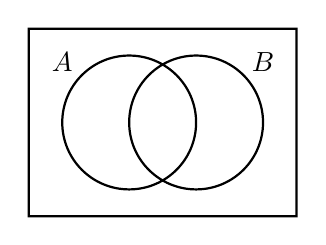
\begin{tikzpicture}[fill=gray!50,scale=0.85]
 \draw[thick] \circleA \circleAlabel \circleB \circleBlabel \twosetbox;
\end{tikzpicture}
}%
\end{sbspanel}%
\begin{sbspanel}{0.34}%
\resizebox{\linewidth}{!}{%
 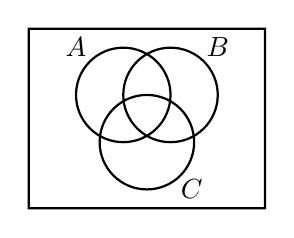
\begin{tikzpicture}[scale=.60, fill=gray!50]
 \draw[thick] \circleA \circleAlabel \circleB \circleBlabel \circleC \circleClabel \threesetbox;
\end{tikzpicture}
}%
\end{sbspanel}%
\end{sidebyside}%
 Each circle represents a set. The rectangle containing the circles represents the universe. To represent combinations of these sets, we shade the corresponding region.
\end{frame}
 
\begin{frame}
\frametitle{}
We can represent \(A \cap B\) as
 \begin{sidebyside}{1}{0.33}{0.33}{0}%
\begin{sbspanel}{0.34}%
\resizebox{\linewidth}{!}{%
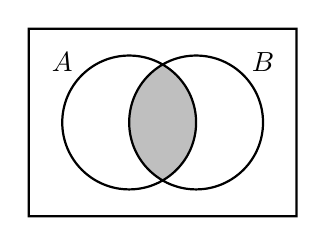
\begin{tikzpicture}[fill=gray!50,scale=0.85]
 	\begin{scope}
 	\clip \circleA;
 	\fill \circleB;
 	\end{scope}
  \draw[thick] \circleA \circleAlabel \circleB \circleBlabel \twosetbox;
 \end{tikzpicture}
}%
\end{sbspanel}%
\end{sidebyside}%
 
\pause \vfill 

We can represent \(A \cap \bar{B} = A \setminus B\) as
 \begin{sidebyside}{1}{0.33}{0.33}{0}%
\begin{sbspanel}{0.34}%
\resizebox{\linewidth}{!}{%
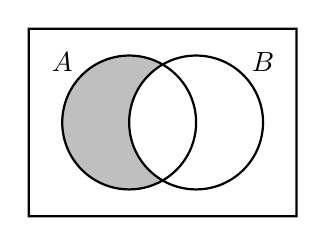
\begin{tikzpicture}[fill=gray!50,scale=0.85]
 	\begin{scope}
 	\clip \twosetbox \circleB;
 	\fill \circleA;
 	\end{scope}
  \draw[thick] \circleA \circleAlabel \circleB \circleBlabel \twosetbox;
 \end{tikzpicture}
}%
\end{sbspanel}%
\end{sidebyside}%
\end{frame}
 
\begin{frame}
\frametitle{}
A more complicated example is \((B \cap C) \cup (C \cap \bar A)\):
 \begin{sidebyside}{1}{0.335}{0.335}{0}%
\begin{sbspanel}{0.33}%
\resizebox{\linewidth}{!}{%
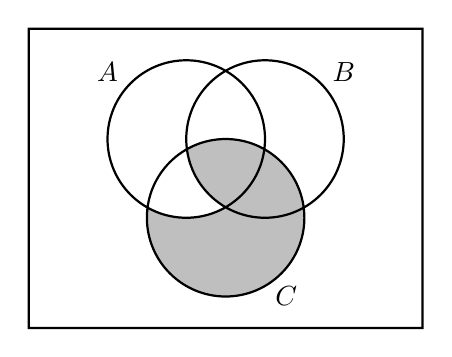
\begin{tikzpicture}[fill=gray!50,scale=1]
 	\fill \circleC;
 	\begin{scope}
 	    \clip \circleC;
 	    \fill[white] \circleA \circleB;
 	  \end{scope}
 	  \begin{scope}
 	  	\clip \circleC;
 	  	\fill \circleB;
 	  \end{scope}
  \draw[thick] \circleA \circleAlabel \circleB \circleBlabel \circleC \circleClabel \threesetbox;
 \end{tikzpicture}
}%
\end{sbspanel}%
\end{sidebyside}%
 Can you describe the shaded region another way?
\end{frame}
 

\end{document}
